% Judul dokumen
\title{Proposal TA}
\author{Pahlevy, Achmad}

% Pengaturan ukuran teks dan bentuk halaman dua sisi
\documentclass[10pt,twoside]{article}


% Pengaturan ukuran halaman dan margin
\usepackage[a4paper,top=25mm,left=25mm,right=20mm,bottom=25mm]{geometry}

% Pengaturan ukuran spasi
\usepackage[singlespacing]{setspace}

% Pengaturan format bahasa
%\usepackage[indonesian]{babel}

% Pengaturan detail pada file PDF
%\usepackage[pdfauthor={\@author},bookmarksnumbered,pdfborder={0 0 0}]{hyperref}

% Pengaturan jenis karakter
\usepackage[utf8]{inputenc}

% Pengaturan pewarnaan
\usepackage[table,xcdraw]{xcolor}

% Pengaturan kutipan artikel
\usepackage[numbers]{natbib}

% Package lainnya
\usepackage{changepage}
\usepackage{enumitem}
\usepackage{eso-pic}
\usepackage{etoolbox}
\usepackage{graphicx}
\usepackage{lipsum}
\usepackage{lmodern}
\usepackage{longtable}
\usepackage{tabularx}
\usepackage{wrapfig}
\usepackage{amssymb}
\usepackage{verbatim}
\usepackage{natbib}

% Definisi untuk "Hati ini sengaja dikosongkan"
\patchcmd{\cleardoublepage}{\hbox{}}{
  \thispagestyle{empty}
  \vspace*{\fill}
  \begin{center}\textit{[Halaman ini sengaja dikosongkan]}\end{center}
  \vfill}{}{}

% Pengaturan penomoran halaman
\usepackage{fancyhdr}
\fancyhf{}
\renewcommand{\headrulewidth}{0pt}
\pagestyle{fancy}
\fancyfoot[CE,CO]{\thepage}
\patchcmd{\chapter}{plain}{fancy}{}{}
\patchcmd{\chapter}{empty}{plain}{}{}


% Pengaturan format potongan kode
\usepackage{listings}
\definecolor{comment}{RGB}{0,128,0}
\definecolor{string}{RGB}{255,0,0}
\definecolor{keyword}{RGB}{0,0,255}
\lstdefinestyle{codestyle}{
  commentstyle=\color{comment},
  stringstyle=\color{string},
  keywordstyle=\color{keyword},
  basicstyle=\footnotesize\ttfamily,
  numbers=left,
  numberstyle=\tiny,
  numbersep=5pt,
  frame=lines,
  breaklines=true,
  prebreak=\raisebox{0ex}[0ex][0ex]{\ensuremath{\hookleftarrow}},
  showstringspaces=false,
  upquote=true,
  tabsize=2,
}
\lstset{style=codestyle}

% Isi keseluruhan dokumen
\begin{document}

  % Atur ulang penomoran halaman
  \setcounter{page}{1}

  % Pengaturan ukuran indentasi paragraf
  \setlength{\parindent}{2em}

  % Pengaturan ukuran spasi paragraf
  \setlength{\parskip}{1ex}

  % Nomor halaman pembuka dimulai dari sini
  \pagenumbering{roman}

  % Abstrak Bahasa Indonesia
  \begin{center}
  \large\textbf{ABSTRAK}
\end{center}

\vspace{2ex}

\begingroup
  % Menghilangkan padding
  \setlength{\tabcolsep}{0pt}

  \noindent
  \begin{tabularx}{\textwidth}{l >{\centering}m{2em} X}
    % Ubah kalimat berikut dengan nama mahasiswa
    Nama Mahasiswa    &:& Achmad Pahlevy Aminullah Nizaruddin \\
    NRP	&:& 0721 18 4000 0001 \\
    Semester	&:& Ganjil 2021 / 2022 \\

    % Ubah kalimat berikut dengan judul tugas akhir
    Judul Tugas Akhir &:&	Sistem Monitoring dan Otomasi Proses Sipon Berbasis IoT dengan menggunakan ESP32 Untuk  Tambak Udang Vaname \\
	& & \textbf{\emph{Monitoring and Automated Syphon System Based On IoT with ESP32 For Vaname Shrimp Pond}} \\

    % Ubah kalimat-kalimat berikut dengan nama-nama dosen pembimbing
    Pembimbing        &:& 1. Arief Kurniawan, S.T., M.T. \\
                      & & 2. Dion Hayu Fandiantoro , S.T., M.Eng. \\
    \underline{Uraian Tugas Akhir}	&:&
  \end{tabularx}
\endgroup


% Ubah paragraf berikut dengan abstrak dari tugas akhir
\vspace{0.5cm}
\noindent
Pada sistem budidaya udang, suhu air dan pH merupakan beberapa indikator penting dalam keberlanjutan budidaya tersebut sehingga penting untuk dipantau. Selain itu, limbah sisa yang mengendap di dasar kolam mempengaruhi kualitas air. Oleh karena itu , terdapat kebutuhan untuk membersihkan residu ini secara teratur untuk menjaga kualitas air dalam kondisi baik. Sampai saat ini, kebanyakan proses sipon masih menggunakan cara tradisional sehingga membutuhkan waktu yang relatif lama. Maka dari itu, diperlukan sistem yang dapat melakukan proses sipon secara otomatis dan juga melakukan monitoring kualitas air, kedua kemampuan pada sistem tersebut bertujuan untuk mempermudah proses sipon serta pemantauan kualitas air. Sistem ini menggunakan microcontroller ESP32 yang menggunakan komunikasi WiFi, kemudian hasil komunikasi atau output yang berupa data sensor  akan disalurkan ke website. Adapun website dalam sistem ini berfungsi untuk menampilkan hasil monitoring kualitas air serta mengatur otomasi proses sipon seperti pengaturan jadwal sipon, durasi sipon, dan sejenisnya.

\vspace{1.5cm}
\begin{center}
  \begin{minipage}{.45\linewidth}
    \begin{flushleft}
	\begin{center}
      \textbf{Dosen Pembimbing I} \\
      \vspace{1.5cm}
       \underline{ Arief Kurniawan, S.T., M.T.} \\
	NIP. 1197409072002121001
	\end{center} 
    \end{flushleft}
  \end{minipage}
  \hfill
  \begin{minipage}{.45\linewidth}
    \begin{flushleft}
	\begin{center}
      \textbf{Dosen Pembimbing II} \\
      \vspace{1.5cm}
       \underline{Dion Hayu Fandiantoro , S.T., M.Eng.} \\
	NPP. 1994202011064
	\end{center} 
    \end{flushleft}
  \end{minipage}
\end{center}

\vspace{1cm}

\begin{center}
  \begin{minipage}{.50\linewidth}
	\begin{center}
      \textbf{Mengetahui,} \\
	\textbf{Departemen Teknik Komputer FTEIC - ITS} \\
	\textbf{Kepala,}\\
      \vspace{1.5cm}
       \underline{ Dr. Supeno Mardi Susiki Nugroho, S.T., M.T.} \\
	NIP. 197003131995121001
	\end{center} 
  \end{minipage}
\end{center}
\cleardoublepage

  % Nomor halaman isi dimulai dari sini
  \pagenumbering{arabic}

%\let\clearpage\relax% Don't allow page break
\begin{center}
\noindent \huge Sistem Monitoring dan Otomasi Proses Sipon berbasis IoT dengan menggunakan ESP32
\end{center}

\section{PENDAHULUAN}

% Ubah bagian-bagian berikut dengan isi dari pendahuluan

\subsection{Latar Belakang}
\label{sec:latarbelakang}

Udang merupakan salah satu komoditas unggulan dunia, yang berarti komoditas tersebut mempunyai prospek yang besar pada sector perikanan, hal tersebut tentunya dapat meningkatkan devisa negara melalui ekspor komoditas perikanan. Tingginya permintaan udang dari dalam dan luar negeri memjadikan Indonesia sebagai salah satu pengirim udang terbesar di dunia[2]. Adapun salah satu jenis udang yang paling banyak diminati di dunia adalah Udang Vanname. Alasannya antara lain adalah Udang Vanname mampu hidup di perairan yang memiliki salinitas rendah sampai tinggi, dan juga dapat beradaptasi dengan lingkungan yang bersuhu rendah, serta mempunyai kelangsungan hidup yang tinggi[3]. Jenis Udang Vaname memiliki nafsu makan yang relative tinggi dan mempunyai kemampuan untuk memanfaatkan pakan dengan kadar protein yang rendah sehingga pemberian pola pakan dapat disesuaikan dengan budidaya tambak[5]. Kemampuan tersebut yang menimbulkan kecocokan bagi pengusaha tambak untuk membudidayakan jenis udang tersebut[4]. \\

Suhu dan pH merupakan beberapa indicator dari keberlanjutan budidaya udang vaname sehingga penting untuk dipantau. Untuk indikator suhu, penting dilakukan pengukuran untuk mengetahui karakteristik perairan, yang mana indikator tersebut adalah faktor abiotik yang memegang peranan penting bagi kehidupan organisme di perairan, Adapun suhu optimal bagi udang berkisar antara 29-32°C[12]. Pada indicator pH, pengupayaan untuk mempertahankan PH air dalam budidaya tambak udang menjadi suatu kewajiban supaya kualitas air dapat terjaga dengan baik dan stabil. Selain itu, konsentrasi pH air berpengaruh terhadap nafsu makan udang serta reaksi kimia dalam air, dan juga apabila konsentrasi pH air dibawah batas toleransi, udang akan menjadi sulit untuk mengganti kulit yang mana akan menjadi lembek sehingga sintasan rendah[13]. pH optimal bagi udang berkisar antara 7,0 – 8,5[12]. \\

Pada sistem budidaya udang vaname, limbah sisa yang mengendap di dasar kolam mempengaruhi kualitas air. Oleh karena itu , terdapat kebutuhan untuk membersihkan residu ini secara teratur untuk menjaga kualitas air dalam kondisi baik. Proses pembersihan residu dinamakan Proses Sipon. Proses sipon pada umumnya mengambil kotoran (sisa pakan maupun feses) dari dasar tambak atau kolam udang dengan menggunakan selang yang menyedot kotoran. \\

Seiring berkembangnya zaman, tidak sedikit pekerjaan manusia yang terbantu dengan adanya teknologi, baik berupa mesin ataupun robot yang mampu bekerja secara otomatis. Sama halnya pada bidang perikanan, khususnya budidaya, contoh yang umum adalah seperti mesin pakan otomatis, yang mana mesin tersebut mampu memberikan pakan secara otomatis dengan mengatur jadwal yang telah ditentukan oleh pengusaha tambak[6]. Pekerja diberikan fasilitas control tersebut dengan tujuan untuk memudahkan dalam pemberian pakan udang, yang mana pakan udang yang diberikan disesuaikan dengan kondisi kebutuhan pakan udang (shrimp feed requirements) agar endapan dari sisa pakan di dasar tidak terlalu banyak[7]. \\

Dalam tugas akhir ini juga melakukan hal yang sama yakni mempermudah pekerjaan manusia khususnya petambak udang dalam membersihkan dasar tambak udang dari endapan sisa makanan yang dapat menyebabkan penurunan kualitas air, dan juga untuk mengawasi kualitas air tambak yang sama dengan melakukan monitoring melalui website. Sistem dan Alat yang dibuat akan menggantikan pekerjaan pembersihan dasar tambak yang pada umumnya dilakukan oleh pekerja tambak yang menyedot kotoran di tambak secara langsung seperti yang dijelaskan sebelumnya, serta mempermudah dalam pemantauan kualitas air tambak. \\



\subsection{Permasalahan}
\label{sec:permasalahan}

Berdasarkan latar belakang tersebut dapat diketahui bahwa untuk mengetahui status keberlanjutan budidaya tambak udang vaname, diperlukan pemantauan suhu dan pH air, selain itu sebagian besar proses sipon masih menggunakan cara yang tradisional yang mana membutuhkan waktu yang lama dan hasil yang tentunya tidak maksimal. \\

\noindent Oleh karena itu, diperlukan sebuah sistem untuk melakukan manajemen otomasi dan monitoring kualitas air sehingga proses sipon dapat dilakukan secara efektif dan efisien.

\subsection{Penelitian Terkait}
\label{sec:Penelitian Terkait}

Dalam penelitian yang dilakukan oleh saudara Indra Jaya dan M Iqbal dari Marine Science and Technology, Faculty of Fisheries and Marine Sciences, IPB University[14]. Dilakukan pembuatan alat yang melakukan proses sipon secara otomatis, yang mana instrument yang digunakan memanfaatkan prinsip equilibrium antara alat utama yang berbentuk piramida dengan alat bantu berupa penyimpan air (water container).

\subsection{Gap Penelitian}
\label{sec:Gap Penelitian}

Dalam penelitian yang dilakukan oleh saudara Indra Jaya dan M Iqbal[14], belum dilakukan pengintegrasian antara alat dengan end device, baik  berupa web yang mana dapat melakukan pengaturan mengenai berapa lama waktu sipon, jadwal sipon yang dilakukan, serta monitoring kualitas air.

\subsection{Tujuan Penelitian}
\label{sec:Tujuan Penelitian}

Membuat sistem yang melakukan monitoring kualitas air dan proses sipon secara otomatis dan dapat dipantau serta diatur melalui web.


\section{TINJAUAN PUSTAKA}

% Ubah bagian-bagian berikut dengan isi dari pendahuluan

\subsection{ESP32}
\label{sec:esp32}
% Ubah bagian-bagian berikut dengan isi dari tinjauan pustaka

ESP32 merupakan mikrokontroller dengan Wi-Fi dan Bluetooth®. Adapun detail spesifikasi nya adalah sebagai berikut [15] :
\begin{itemize}
	\item Menurut sistem dan memorinya, ESP32 merupakan sistem dual-core (PRO-CPU untuk protocol dan APP-CPU untuk aplikasi) dengan dua CPU Harvard Architecture Xtensa LX6. Kemudian untuk memori tertanamnya, baik memori eksternal maupun peripheral lainnya terletak pada data bus dan/atau pada instruction bus dari CPU tersebut. Space address untuk data dan instruction bus adalah 4GB lalu untuk peripheral space address sebesar 512KB. Kemudian memori tertanamnya sebesar 448KB ROM, 520KB SRAM, dan dua 8KB memori RTC.
	\item Menurut Clock dan Timer nya, ESP32 dapat menggunakan baik Phase Lock Loop (PLL) internal 320MHz maupun kristal eksternal. ESP32 juga memungkinkan untuk penggunaan oscillating circuit sebagai clock source pada 2-40MHz yang menghasilkan master clock CPU-CLK untuk kedua core CPU. Clock ini dapat setinggi 160MHz untuk High Performance atau direndahkan guna mengurangi pemakaian daya (power consumption).
	\item Secara pemrograman, sistem operasi real-time dari ESP32 adalah FreeRTOS, yang mana merupakan sistem operasi open-source. Kemudian Bahasa pemrograman yang umum digunakan pada ESP32 adalah Bahasa C, namun mikrokontroller ini dapat dengan mudah deprogram dengan menggunakan Bahasa C++.
\end{itemize}

\subsection{WiFi}
\label{sec:wifi}

Hotspot (Wi-Fi) adalah satu standar Wireless Netwoking tanpa kabel, hanya dengan komponen yang sesuai dapat terkoneksi ke jaringan\cite{trikun}. Wireless Fidelity (Wi-Fi) merupakan sebuah media penghantar komunikasi data tanpa kabel yang bisa digunakan untuk komunikasi atau mentransfer program dan data dengan kemampuan yang sangat cepat. Wi-Fi juga dapat diartikan teknologi yang memanfaatkan peralatan elektronik untuk bertukar data dengan menggunakan gelombang radio (nirkabel) melalui sebuah jaringan komputer, termasuk koneksi internet berkecepatan tinggi. Istilah Wi-Fi banyak dikenal oleh masyarakat sebagai media untuk internet saja, namun sebenarnya bisa juga difungsikan sebagai jaringan tanpa kabel (nirkabel) seperti di perusahaan-perusahaan besar dan juga di warnet. Jaringan nirkabel tersebut biasa diistilahkan dengan LAN (local area network). Sehingga antara komputer dilokasi satu bisa saling berhubungan dengan komputer lain yang letaknya berbeda. Sedangkan untuk penggunaan internet, Wi-Fi memerlukan sebuah titik akses yang biasa disebut dengan hotspot untuk menghubungkan dan mengontrol antara pengguna Wi-Fi dengan jaringan internet pusat. Sebuah hotspot pada umumnya dilengkapi dengan password yang bisa meminimalisasi siapa saja yang bisa menggunakan fasilitas tersebut. Fitur ini sering digunakan oleh pengguna rumahan, restoran, swalayan, café dan hotel.

\subsection{Node.js}
\label{sec:nodejs}

Merupakan perangkat lunak yang digunakan dalam pengembangan aplikasi berbasis web dengan penulisan dalam sintaks bahasa pemrograman JavaScript. NodeJs dikembangkan untuk menyempurnakan kinerja javascript dalam pemrogaman server seperti PHP, Ruby, Perl, dan sebagainya. Salah satu keuntungan dari NodeJS adalah dapat digunakan di banyak operasi sistem seperti Windows, Mac OS, Linux. Untuk menjalankan server web, NodeJS tidak memerlukan program server web seperti Apache atau Nginx karena telah memiliki pustaka server HTTP tersendiri[18].

\subsection{HTML}
\label{sec:html}

HTML (Hypertext Markup Language) merupakan sarana untuk memberi tahu web browser cara menampilkan halaman jejaring (webpage)[10]. HTML menentukan syntax serta penempatan direksi embedded khusus yang tidak ditampilkan oleh peramban (browser) tetapi memberikan saran mengenai cara menampilkan konten dari dokumen, termasuk teks, gambar, serta media pendukung yang lainnya. HTML juga membuat dokumen menjadi lebih interaktif melalui hypertext link special, yang mana menghubungkan dokumen terkait dengan dokumen lain di komputer serta sumber dari internet[11]. 

\subsection{MQTT}
\label{sec:mqtt}

MQTT (Message Queuing Telemetry Transport) merupakan suatu protokol konektifitas  dari mesin ke mesin / machine to machine (M2M) yang memiliki kemampuan untuk mengirimkan data dengan sangat ringan menggunakan arsitektur TCP/IP [8]. Pada MQTT sendiri mempunyai keunggulan yaitu dapat mengirimkan data dengan bandwith yang ringan, konsumsi listrik yang sedikit, latensi serta konektifitas yang sangat tinggi, ketersediaan variable yang banyak serta jaminan pengiriman data yang dapat dinegosiasikan.

\subsection{MongoDB}
\label{sec:mongodb}

Merupakan kategori database NoSQL yang sedang dikembangkan secara aktif oleh 10gen menjadi MongoDB I.inc. MongoDB sendiri open-source yang sumbernya tersedia di banyak platform seperti Github. Fitur yang dimiliki MongoDB yaitu JSON-friendly database yang berarti dokumen yang disimpan ataupun diterima dari MongoDB sebagai objek JavaScript. Fitur yang berikutnya adalah schemaless nature, yang intinya adalah tidak perlu mendefinisikan struktur dari data yang disimpan (schema). MongoDB juga memperkenalkan konsep sharding, yang mana memungkinkan untuk melakukan scaling database secara horizontal serta vertikal[9].

\subsection{Suhu dan Temperatur pada Budidaya Udang Vaname}
\label{sec:suhudantemperatur}

Dalam budidaya udang vaname,, kualitas air merupakan salah satu faktor utama yang menentukan keberhasilan dari proses budidaya, terdapat banyak parameter yang digunakan dalam pengukuran kualitas air seperti Suhu, pH, Salinitas, DO, Kecerahan,
Nitrit, Fosfat, Alkalinitas, Besi(Fe), H2S, dan Jumlah Patogen. Adapun parameter yang akan dimonitoring dalam sistem adalah Suhu dan pH. Dalam parameter suhu, nilai optimal pada budidaya tambak udang adalah 26-32°C, range tersebut akan berdampak pada metabolisme udang serta laju pencernaan yang mana akan mempengaruhi pertumbuhan udang. Apabila dibawah 26°C, metabolisme udang akan menurun sehingga pertumbuhan udang terhambat, sedangkan jika diatas 32°C, enzim akan rusak [16]. Sedangkan dalam parameter pH, kadar yang ideal dalam tambak adalah 7,5-8,5. Apabila pH terlalu asam (<7,5) akan menyebabkan tingginya resiko penyakit dan tingkat kematian udang serta menipisnya oksigen terlarut akibat terikat mineral[17].

\section{METODOLOGI}

% Ubah bagian-bagian berikut dengan isi dari pendahuluan

\subsection{Data dan Peralatan/ Data dan Alat Bantu/ Material }
\label{sec:datadanperalatan}

\textbf{Hardware}
\begin{enumerate}[label=(\alph*)]
   \item ESP32
% Contoh input gambar
\begin{figure}[ht]
  \centering

  % Ubah dengan nama file gambar dan ukuran yang akan digunakan
  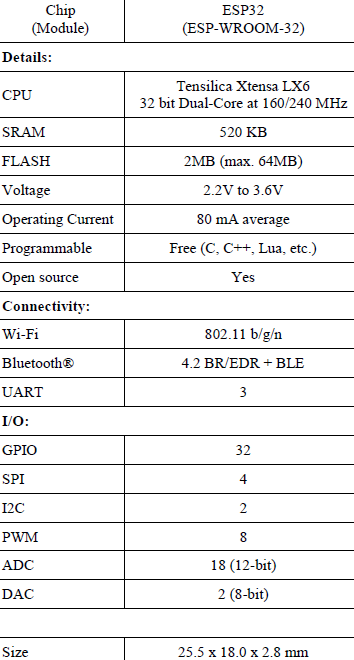
\includegraphics[scale=0.5]{gambar/tabelsatuu.png}

  % Ubah dengan keterangan gambar yang diinginkan
  \caption{Spesifikasi ESP32 }%\citep{roketluarangkasa}.}
  \label{fig:tabelsatu}
\end{figure}
	\item Relay Pompa
	\begin{itemize}
		\item Tipe : MK2P-1
		\item Volt : 220 V AC 10 A
	\end{itemize}
	\item DS18B20 Digital Temperature Sensor
	\begin{itemize}
		\item Operating voltage: 3.0~ 5.5V
		\item ±0.5°C Akurasi dari -10°C ke +85°C
		\item Usable temperature range: -55 to 125°C (-67°F to +257°F)
		\item Query time kurang dari 750ms
		\item Diameter Kabel: 4mm(0.16")
		\item Panjang: 90cm(35.43")
	\end{itemize}
	\item pH Meter Sensor dengan Modul PH-4502C (Analog)
	\begin{itemize}
		\item Heating voltage : 5 ± 0.2V (AC · DC)
		\item Working current : 5-10mA
		\item Range konsentrasi yang dapat dideteksi : PH 0-14
		\item Range deteksi suhu : 0-80 °
		\item Waktu respon :  $\leq 5S$
		\item Settling Time : $\leq 60S$
		\item Daya Komponen : $\leq 0.5W$
		\item Ukuran Modul: 42mm × 32mm × 20mm
		\item Output: analog voltage signal output
	\end{itemize}
	\item Converter Tegangan \\
	AC-DC Konverter Adaptor
	\begin{itemize}
		\item	Input AC : 220V +/- 15 \%
		\item	Output DC : 12V ~ 2A
		\item	Berat : 200gr
		\item	Tipe Connector 5,5mm
		\item	Panjang Kabel 100cm
	\end{itemize}
\vspace{0.5cm}
	DC-DC Step-Down Konverter
	\begin{itemize}
	\item Voltase Input : 4.75V-23V
	\item Voltase Output: 1.0V-17V
	\item Arus Output : menurunkan nilai 3A, panjang 1.8A
	\item Efisiensi Konversi : 96\% (maksimum)
	\item Frekuensi Switching : 340KHz
	\item Load regulation: ±0.5 \%
	\item Voltage regulation: ±2.5 \%
	\item Dimensi Eksternal: 17 * 11 * 3.8 (P * L * T) (mm
	\end{itemize}
	\item Converter ADC eksternal (ADS1115)
	\begin{itemize}
	\item Resolusi: 16 Bits
	\item Programmable Sample Rate: 8 to 860 Samples/Detik
	\item Power Supply : 2.0V to 5.5V
	\end{itemize}
	\item Laptop dengan spesifikasi :
	\begin{itemize}
	\item Prosesor AMD Ryzen 5 5500U dengan Radeon Graphics (12CPUs), ~2.1GHz
	\item Memory RAM 8192 MB
	\end{itemize}
	Penggunaan Laptop adalah untuk pemrograman mikrokontroller, website, dan pembuatan model prototipe tambak (akuarium kustom)
	\item Pompa Submersibel Akuarium (2 buah)
	\begin{itemize}
	\item Tegangan : 220-240V
	\item Daya : 5 Watt
	\item HMax : 90Cm
	\item Output : 380L/Jam
	\item Diameter Outlet : 1/2 inch
	\end{itemize}
\end{enumerate}

\textbf{Software}
\begin{itemize}
	\item Arduino IDE
	\item Visual Studio Code
	\item AutoCad Fusion360
\end{itemize}

\textbf{Material}
\begin{itemize}
	\item Kaca untuk Prototipe Tambak berupa Akuarium Kustom (100 cm x 100 cm x 30 cm)
	\item Selang standard akuarium (ukuran sekitar 5/6 in)
\end{itemize}

\subsection {Metodologi Penelitian}
\label{sec:metodologipenelitian}


% Contoh input gambar
\begin{figure}[htbp]
  \centering

  % Ubah dengan nama file gambar dan ukuran yang akan digunakan
  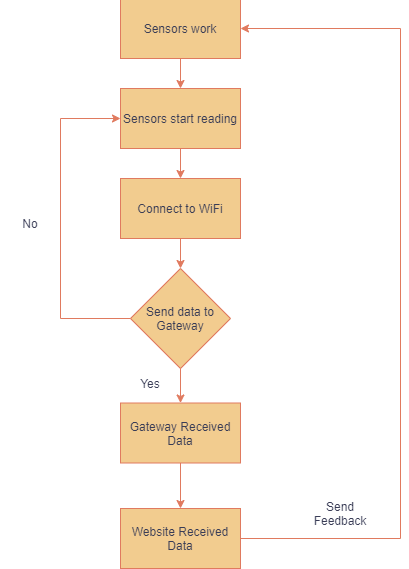
\includegraphics[scale=0.5]{gambar/diagramsatuu.png}

  % Ubah dengan keterangan gambar yang diinginkan
  \caption{Blok Diagram Metodologi Sistem} %  \citep{roketluarangkasa}.}
  \label{fig:diagramsatu}
\end{figure}

% Contoh input gambar
\begin{figure}[htbp]
  \centering

  % Ubah dengan nama file gambar dan ukuran yang akan digunakan
  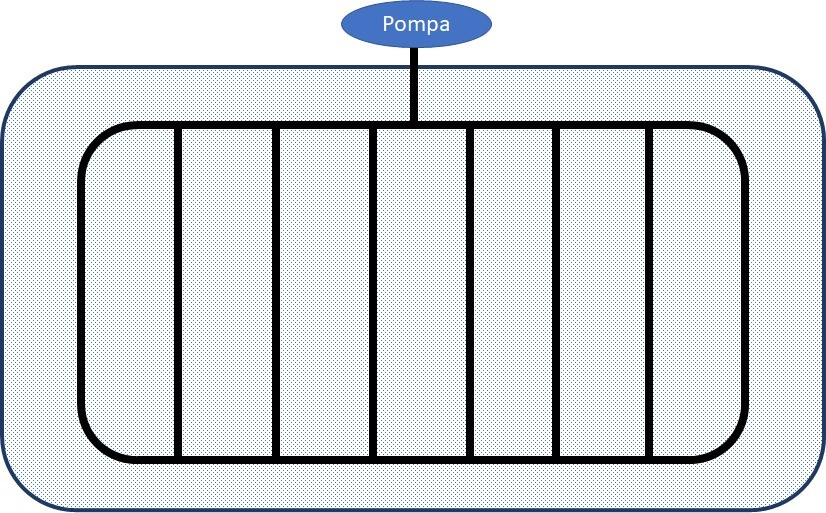
\includegraphics[scale=0.4]{gambar/bentukpipa.jpg}

  % Ubah dengan keterangan gambar yang diinginkan
  \caption{Bentuk Pipa sipon yang digunakan untuk menggantikan pekerjaan petambak}%  \citep{roketluarangkasa}.}
  \label{fig:bentukpipa}
\end{figure}

% Contoh input gambar
\begin{figure}[htbp]
  \centering

  % Ubah dengan nama file gambar dan ukuran yang akan digunakan
  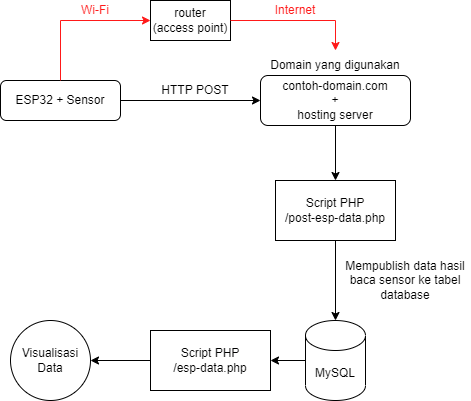
\includegraphics[scale=0.7]{gambar/metodekomunikasi.png}

  % Ubah dengan keterangan gambar yang diinginkan
  \caption{Metode Komunikasi dari Microcontroller ke Web}%  \citep{roketluarangkasa}.}
  \label{fig:metodekomunikasi}
\end{figure}

% Contoh input gambar
\begin{figure}[htbp]
  \centering

  % Ubah dengan nama file gambar dan ukuran yang akan digunakan
  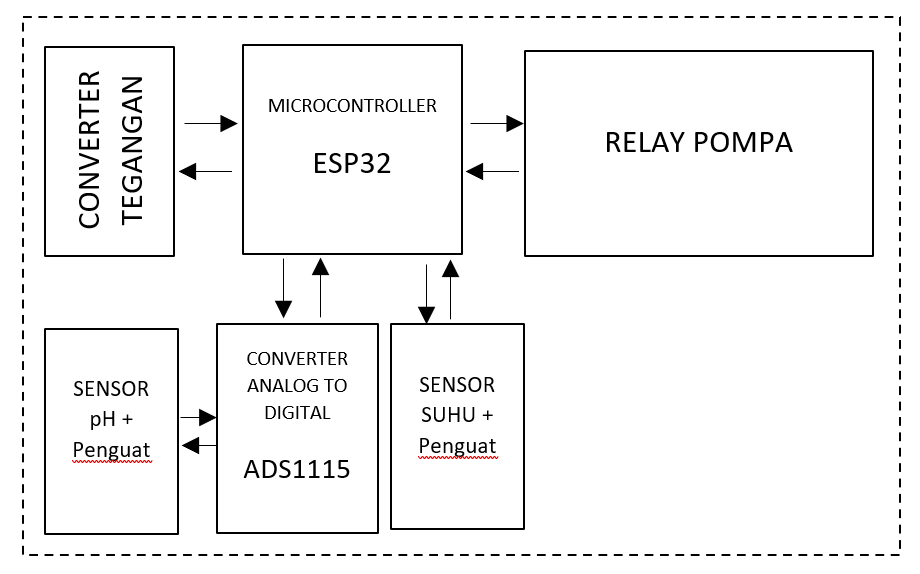
\includegraphics[scale=0.5]{gambar/blok.png}

  % Ubah dengan keterangan gambar yang diinginkan
  \caption{Blok Komponen Alat Sistem Otomasi Sipon dan Monitoring} % \citep{roketluarangkasa}.}
  \label{fig:metodekomunikasi}
\end{figure}



\begin{enumerate}
\item Cara Kerja Sistem \\
Sensor pada alat akan mengambil data yang diperlukan, yang kemudian akan diteruskan menuju Gateway dengan koneksi Wi-Fi pada modul, setelah data diterima Gateway, data akan diteruskan ke website yang mana untuk data sensor akan ditampilkan pada website tersebut. Untuk data relay, website memberikan feedback kepada relay yang nantinya akan menyebabkan relay berfungsi sesuai dengan feedback dari website.
\item Model Pipa \\
Untuk menggantikan metode umum proses sipon yang mana memerlukan petambak untuk mengitari tambaknya (Sebagian besar menggunakan pola S atau ular ), digunakan pipa yang berbentuk sesuai dengan ilustrasi diatas (gambar 2), dengan keterangan kotak biru sebagai tambak, titik biru sebagai air, kemudian garis hitam sebagai pipa (diameter sekitar 1in). Samping pipa akan diberi lubang dengan diameter 2 – 5 cm yang kemudian akan diletakkan pada dasar tambak, dengan tujuan dapat menyedot keseluruhan air dengan merata.
\item Website \\
Untuk komunikasi antara alat dengan website, menggunakan koneksi Wi-Fi yang mana sudah terpasang pada modul, kemudian menggunakan protokol MQTT untuk mengirimkan data pada domain website, lalu data akan disimpan pada database dengan menggunakan MongoDB, setelah itu dengan memanfaatkan websocket, node.js, dan vue.js, data akan divisualisasikan pada website. Sedangkan untuk komunikasi dari website menuju relay hampir identik dengan alur sebelumnya, hanya saja dimulai dari website dan  berakhir ke relay atau aktuator itu sendiri.
\item Alat Pada Sistem \\
Dalam alat yang  akan digunakan pada sistem, terdapat komponen seperti  converter tegangan, Microcontroller ESP32 dengan build-in Wi-Fi, Relay Pompa, Sensor pH dan sensor temperatur dengan modul penguatnya masing – masing,  serta konverter analog ke digital (ADS1115) untuk menghubungkan mikrokontroller dengan sensor yang masih analog.
\end{enumerate}
\section{HASIL YANG DIHARAPKAN}

Sistem yang dapat melakukan proses sipon secara otomatis serta memonitoring kualitas air tambak, yang kemudian dapat dipantau atau diatur melalui website.
\section{RENCANA KERJA}
\begin{figure}[ht]
  \centering

  % Ubah dengan nama file gambar dan ukuran yang akan digunakan
  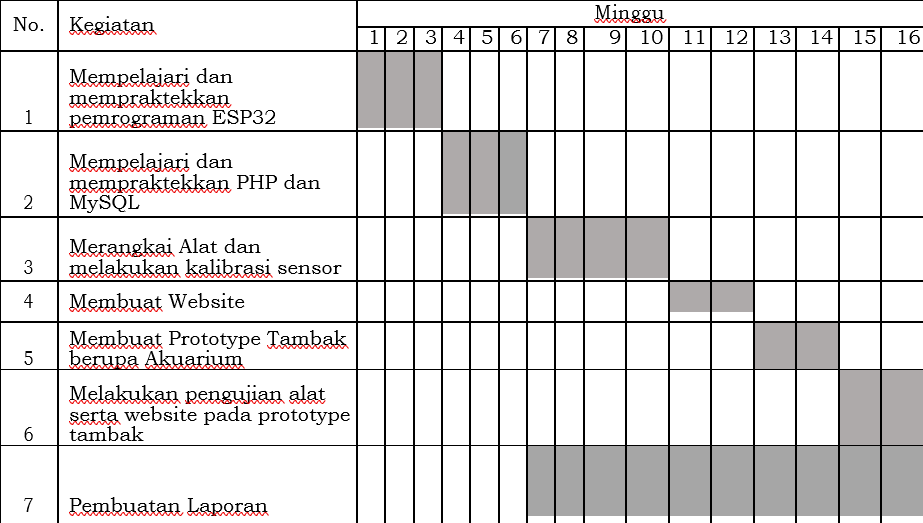
\includegraphics[scale=0.7]{gambar/rencana.png}

  % Ubah dengan keterangan gambar yang diinginkan
  \label{fig:rencana}
\end{figure}
 \renewcommand\refname{DAFTAR PUSTAKA}
 \bibliographystyle{ieeetr}
 \bibliography{pustaka/daftarpustaka.bib}
 \cleardoublepage


\end{document}
